%
% Template for DAS course projects
%
\documentclass[a4paper,11pt,oneside]{book}
\usepackage[latin1]{inputenc}
\usepackage[english]{babel}
\usepackage{amsfonts}
\usepackage{amsmath}
\usepackage{amssymb,amsmath,color}
\usepackage{graphicx}
\graphicspath{{./figs/}}
\usepackage{subcaption}
\usepackage{float}
\usepackage{tikz}
\usepackage{listofitems} % for \readlist to create arrays
\usepackage[outline]{contour} %
\usepackage{xcolor}

\tikzstyle{node}=[thick,circle,draw=blue,minimum size=22,inner sep=0.5,outer sep=0.6]
\tikzstyle{bias}=[thick,square,draw=black,minimum size=22,inner sep=0.5,outer sep=0.6]
\tikzstyle{node in}=[node,green!20!black,draw=green!30!black,fill=green!25]
\tikzstyle{node hidden}=[node,blue!20!black,draw=blue!30!black,fill=blue!20]
\tikzstyle{node out}=[node,red!20!black,draw=red!30!black,fill=red!20]
\tikzstyle{connect}=[thick,black] 
\tikzset{ % node styles
  node 1/.style={node in},
  node 2/.style={node hidden},
  node 3/.style={node out},
}
\def\nstyle{int(\lay<\Nnodlen?min(2,\lay):3)} % map layer number onto 1, 2, or 3

\usepackage{hyperref}
\hypersetup{
    colorlinks,
    citecolor=black,
    filecolor=black,
    linkcolor=blue,
    urlcolor=black
}


\begin{document}
\pagestyle{myheadings}

%%%%%%%%%%% Cover %%%%%%%%%%%
\thispagestyle{empty}                                                 
\begin{center}                                                            
    \vspace{5mm}
    {\LARGE UNIVERSIT\`A DI BOLOGNA} \\                       
      \vspace{5mm}
\end{center}
\begin{center}
  
\includegraphics[scale=.27]{logo_unibo}
\end{center}
\begin{center}
      \vspace{5mm}
      {\LARGE School of Engineering} \\
        \vspace{3mm}
      {\Large Master Degree in Automation Engineering} \\
      \vspace{20mm}
      {\LARGE Distributed Autonomous Systems} \\
      \vspace{5mm}{\Large\textbf{DISTRIBUTED CLASSIFICATION VIA NEURAL NETWORKS AND FORMATION CONTROL}}                  
      \vspace{15mm}
\end{center}
\begin{flushleft}                                                                              
     {\large Professors:}\\
     \textbf{\@ Giuseppe Notarstefano} \\
     \textbf{\@ Ivano Notarnicola} \\        
     \vspace{13mm}
\end{flushleft}
\begin{flushright}
      {\large Students:}\\
      {Simone Cenerini} \\
      {Giulia Cutini} \\
      {Riccardo Paolini} \\
\end{flushright}        %capoverso allineato a destra
\begin{center}
\vfill
      {\large Academic year \@2022/2023} \\
\end{center}



\newpage
\thispagestyle{empty}

%%%%%%%%%%% Abstract %%%%%%%%%%%%
\begin{center}
\chapter*{}
\thispagestyle{empty}
{\Huge \textbf{Abstract}}\\
\vspace{15mm}
\end{center}

The report shows the development of two projects that aim to show the application of distributed control algorithms in different fields.

\bigskip
The report is organized as follows: in the first chapter we describe the distributed implementation of a binary classification task for images of handwritten digits. The aim is to run in parallel several neural networks by different agents that communicate only locally with neighbors, and thanks to a distributed algorithm we expect them to obtain the same performances on a common test set. We show different test we have tried, such as how the accuracy changes by changing the target digit or how the type of graph changes the epochs required to reach consensus among agents.

\bigskip
In the second chapter we describe the ROS2 implementation of the distance-based formation control law by exploiting also several possible scenarios such as the collision avoidance, the moving formation and the obstacle avoidance. 
We have done different test in order to validate the implementation using different target shapes both in 2d and in 3d, in by giving to the leaders different inputs, also in order to achive a target position.

\tableofcontents \thispagestyle{empty}
% \listoffigures\thispagestyle{empty}

%%%%%%%%%% Introduction %%%%%%%%%%
%\chapter*{Introduction}
%\addcontentsline{toc}{chapter}{Introduction}
%\section*{Motivations} 
%
%\section*{Contributions}



%%%%%%%%%% Chapter Title %%%%%%%%%%
%%%%%%%%%% Chapter Title %%%%%%%%%%
\chapter{Distributed classification via Neural Network}

\begin{figure}
	\centering
	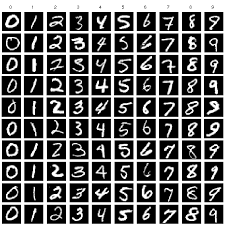
\includegraphics[scale=0.5]{mnist}
	\caption{Example of images from the \texttt{mnist} dataset}
	\label{mnist}
\end{figure}


In the first task we were asked to correctly classify a set of grayscale images. The dataset, downloaded from the Keras \texttt{mnist}, collects images of hand-written digits of $28\times28$ pixels each one, an example in figure \ref{mnist}. In order to perform our task we were asked to implement a distributed classification: given a predefined number of agents running each one a neural network with the same structure, we were asked to implement a Gradient Tracking algorithm to ensure consensus of the connection weights of the several neural networks runned separately by different agents.

\section{Initial setup}
The first step was to prepare the dataset by a reshape and a normalization of the images. We have flattened the $28\times28$ pixels grayscale images in order to obtain a $[784,1]$ column vector and we have normalized the pixels' intensities by dividing each intensity by $255$ in order to avoid a saturation of the activation function.

The classification we were asked to perform was a binary one: we have choose one among the ten digits (named as \texttt{target}) and assigned to it the label $1$, while, to all the other images, we have assigned the label $0$, in the following way:
\begin{equation}
y_i = 
\begin{cases}
1, & \text{if label = \texttt{target}} \\
0, & \text{otherwise}
\end{cases}
\end{equation}

As a consequence, we have performed a \textbf{balancing of the dataset}: in order to efficiently train our neural network we have equalized the representation of both the classes in the dataset ($50 \%$ of both since we have two classes). In order to do that we have undersampled the number of samples in the majority class. 

\section{Neural Network structure}

% NEURAL NETWORK SCHEME
\begin{figure}
\centering
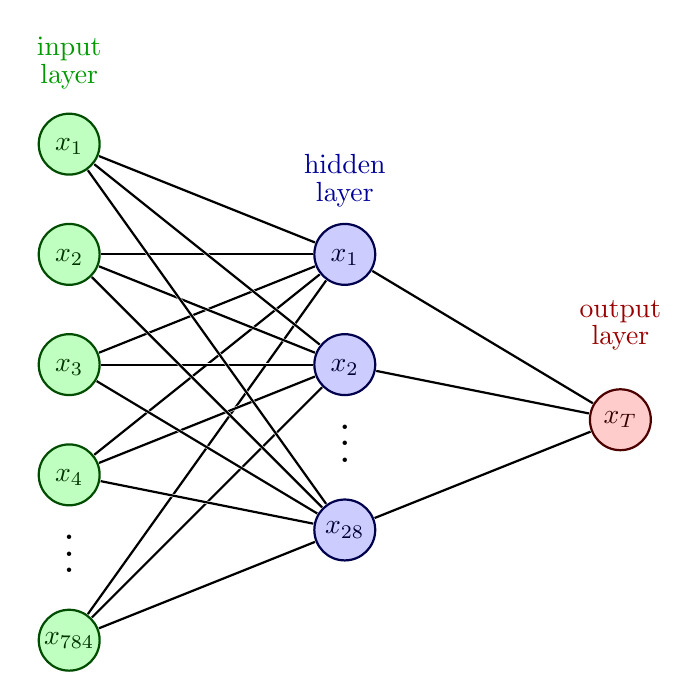
\begin{tikzpicture}[x=3.5cm,y=1.4cm]

\readlist\Nnod{5,3,1} % array of number of nodes per layer
\readlist\Nstr{n,m,k} 
\readlist\Cstr{\strut x,\strut x,{}} 
\def\yshift{0.5} % shift last node for dots


\foreachitem \N \in \Nnod{ 
\def\lay{\Ncnt} 
\pgfmathsetmacro\prev{int(\Ncnt-1)}
\message{\lay,}
\foreach \i [evaluate={\c=int(\i==\N); \y=\N/2-\i-\c*\yshift;
\index=(\i<\N?int(\i):"\Nstr[\lay]");
\x=\lay; \n=\nstyle;}] in {1,...,\N}{


% NODES
\ifnum\lay=1 % First Layer
  \ifnum\i=\N % Last neuron of first layer
    \node[node \n] (N\lay-\i) at (\x,\y) {$x_{784}$}; 
  \else
    \node[node \n] (N\lay-\i) at (\x,\y) {$\Cstr[\lay]_{\index}$};
  \fi
\fi

\ifnum\lay=2 % Second Layer
  \ifnum\i=\N % Last neuron of second layer
    \node[node \n] (N\lay-\i) at (\x,\y) {$x_{28}$}; 
  \else
    \node[node \n] (N\lay-\i) at (\x,\y) {$\Cstr[\lay]_{\index}$}; %empty
  \fi
\fi

\ifnum\lay=3 % Third Layer
  \node[node \n] (N\lay-\i) at (\x,\y) {$x_T$}; 
\fi


% CONNECTIONS
\ifnum\lay>1 % connect to previous layer
  \foreach \j in {1,...,\Nnod[\prev]}{ 
    \draw[connect,white,line width=1.2] (N\prev-\j) -- (N\lay-\i);
     \draw[connect] (N\prev-\j) -- (N\lay-\i);
}
\fi % nothing to connect first layer
      
}
\ifnum\lay<\Nnodlen % draw dots for all layers except the last one
    \path (N\lay-\N) --++ (0,1+\yshift) node[midway,scale=1.5] {$\vdots$};
    \fi
}

% LABELS
% \pixel[above=5,align=center,black] at (N1-1.90) {flatten\\[-0.2em]image}
  \node[above=5,align=center,green!60!black] at (N1-1.90) {input\\[-0.2em]layer};
  \node[above=2,align=center,blue!60!black] at (N2-1.90) {hidden \\[-0.2em]layer};
  \node[above=10,align=center,red!60!black] at (N\Nnodlen-1.90) {output\\[-0.2em]layer};
  
\end{tikzpicture}
\caption{Scheme of the neural network for image classification}
\label{NN_scheme}
\end{figure}


The structure we have choose to develop for the neural network is a tapered one, represented in figure \ref{NN_scheme}. 
The first layer is composed by $784$ neurons, that is the dimension of the flattened image we give as input in the network. In this way each neurons of the first layer gets a single pixel as input. The second layer, the hidden one, has $28$ neurons since an higher number of neurons was useless in order to accomplish our task, while it increases a lot the computational effort required to train the network. The last layer has just one single neuron since we are asked to perform a binary classification, and thus only a number between $0$ and $1$ is required as a prediction.

\bigskip
In this setting we obtain two sets of weights, one for the connections between the input and hidden layers, while the second one is for the connections between the hidden and output layers. In particular, each neuron of the generic layer $L^t$ is connected with all the neurons of the previous layer $L^{t-1}$ plus one connection for the bias, thus each set $W^t$ contains $|L^t| * (|L^{t-1}| + 1)$ weights.

\bigskip
The activation function used to introduce non-linearities into the model is the \textbf{sigmoid} function

\begin{equation}
\sigma(x) = \frac{1}{1 + \exp^{-x}}
\end{equation}

and its derivative is

\begin{equation}
\frac{d}{dx}\sigma(x) = \frac{\sigma(x)}{1 - \sigma(x)}
\end{equation}



\section{Training}
The training happens as a sequence of epochs, every epoch contains multiple mini-batches that are small sets of images. For each mini-batch the computations are the following:

\begin{itemize}
    \item Forward pass to compute the prediction;
    \item Loss and gradient evaluation;
    \item Backward pass to compute the derivative of the loss function with respect to each weight of the network.
    \item Weights update.
\end{itemize}

The loss function we used is the \textbf{binary cross-entropy}

\begin{equation}
L = - y_i \cdot log(\hat{y}) - (1 - y_i) \cdot log(1 - \hat{y_i})
\end{equation}

and its derivative with respect to the activations in the output layer, i.e. the prediction, is

\begin{equation}
\frac{\partial L}{\partial \hat{y}} = - \frac{y}{\hat{y}} + \frac{1 - y}{1 - \hat{y}}
\end{equation}

\bigskip 
The initial connection weights for our neural network have been randomly initialized very close to zero, while the bias term has been initialize at $0.5$ since our prediction value will be $\in[0,1]$ 

\subsection{Gradient Tracking algorithm}
The training we were required to implement was a distributed one: several agents run a neural network with the same structure, over a different training set, then thanks to the \textbf{Gradient Tracking algoritm} we make possible to them to reach consensus over the weights.
To implement the Gradient Tracking algorithm we compute the new weights $x^{k+1}$ before the forward pass, contrarily the auxiliary variable $s^{k+1}$ is obtained after the backward pass since its computation requires the gradient computed with the new weights $x^{k+1}$.

\begin {equation}implemented
\begin{split}
x_i^{k+1} &= \sum_{j \in N_i} a_{ij} x_j^k - \alpha s_i^k \\
s_i^{k+1}   &= \sum_{j \in N_i} a_{ij} s_j^k - \nabla f_i(x_i^{k+1}) - \nabla f_i(x_i^k) \\
\end{split}
\end{equation}

The adjacency matrix $A$ from which we extract the coefficient $a_{ij}$ is a non-negative matrix such that the entry $(i,j)$ is $a_{ij}>0$ if $(i,j)$ is and edge of the graph, $a_{ij}=0$ otherwise.
In our implementation we have chose the adjacency matrix weight according to the \textit{Metropolis Hastings} rule:
\begin{equation}
A_{ij} = 
\begin{cases}
\frac{1}{\max\{d_i,d_j\}+1},  &\text{if } (i,j) \in E \text{and} i \neq j, \\
1-\sum_{h \in N_i} A_{ih}, &\text{if }  i=j \\
0, &\text{otherwise}
\end{cases}
\end{equation}

\section{Experiments and Results}
For testing the network we use the test set we created without splitting it, in this way we can check whether the agents provide results that are equal, given that they should reach consensus to the same weights. 

\bigskip
The performance have been evaluated using the accuracy as a metric. In addition, given that the predictions are not binary we threshold them at 0.5.

\begin{equation}
\hat{y}_i = 
\begin{cases}
1, & \hat{y}_i > 0.5 \\
0, & \hat{y}_i \le 0.5
\end{cases}
\end{equation}

We made different experiments to verify the functioning of the network both as the hyper-parameters such as step-size change but also as the target class or graph changes.

\section{First test}
In the first experiment we want to inspect the convergence of the network. In this configuration we have 5 agents communicating according to a \textit{cycle graph} \ref{test1_graph}, each of them is trained on 32 mini-batches containing 8 samples each for a total of 256 images. 

\begin{figure}[h]
    \centering
    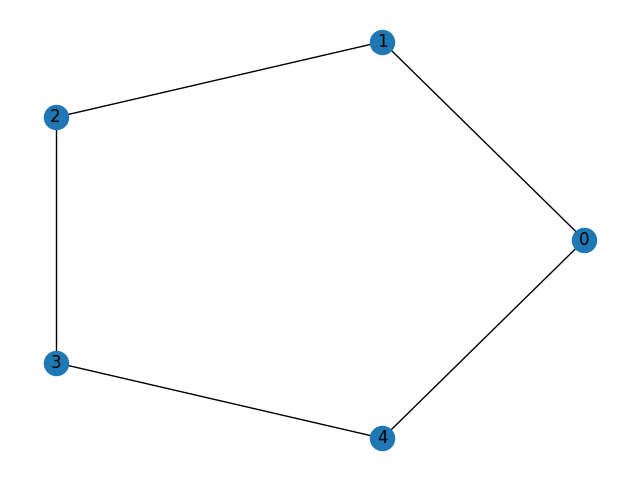
\includegraphics[width=0.32\textwidth]{test1/Graph}
    \caption{Communication graph}
    \label{test1_graph}
\end{figure}

From the plots in \ref{test1_loss} we can appreciate the evolution of the cost function and norm of the gradients, in particular it is possible to observe that the magnitude of the gradients decreases exponentially indicating a fast improvement of the networks.

\begin{figure}[h]
\centering
	\begin{subfigure}{0.49\textwidth}	
	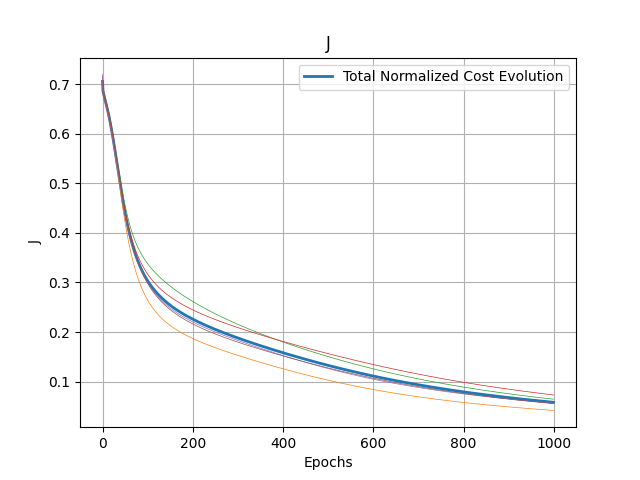
\includegraphics[scale=0.43]{test1/J}
	\caption{Cost evolution}
	\end{subfigure}
\hfill
	\begin{subfigure}{0.49\textwidth}	
	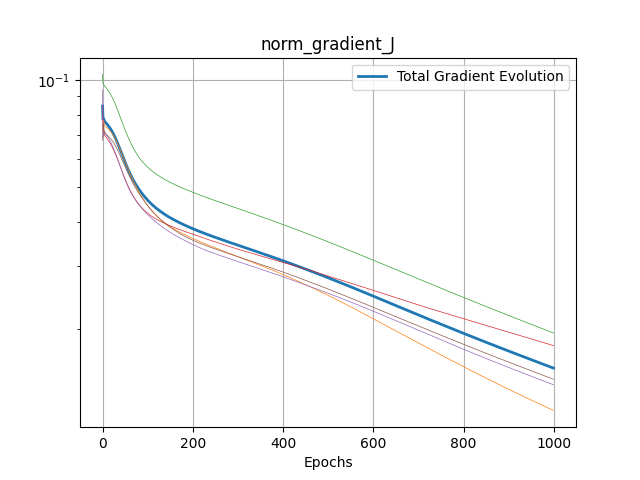
\includegraphics[scale=0.43]{test1/norm_gradient_J}
	\caption{Gradients evolution}
	\end{subfigure}
\caption{Evolution of the cost function and norm of the gradients.}
\label{test1_loss}
\end{figure}

After that, to see if the network converges, we take a single weight from the networks and, for each node, we plot the difference from the mean value of the weight. If the network's weights converge we expect these values to be equal for different nodes, thus they will be equal to the mean and the difference goes to zero. Indeed, from the plot \ref{test1_var}(a) we can see that these differences approaches the zero value, therefore the networks converge to a consensus. However, it can also be observed that in reaching this consensus the weights of the networks oscillate, but these oscillations have smaller and smaller amplitudes \ref{test1_var}(b).

\bigskip
In this experiment we obtained an accuracy of $94.9\%$ on the test set.

\begin{figure}[h]
\centering
	\begin{subfigure}{0.49\textwidth}	
	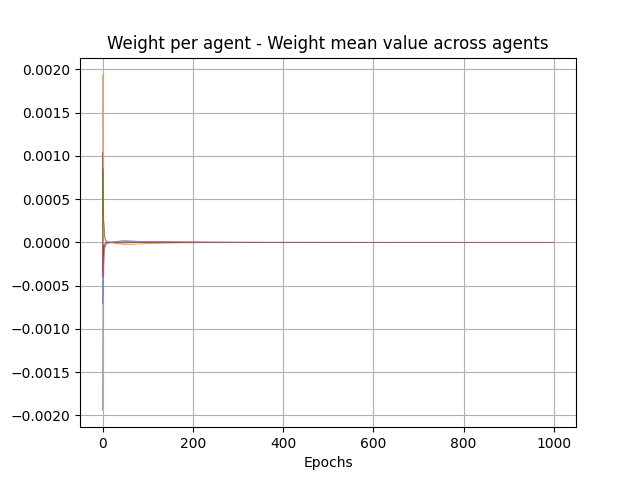
\includegraphics[width=\textwidth]{figs/test1/Single_weight}
	\caption{Weight evolution}
	\end{subfigure}
\hfill
	\begin{subfigure}{0.49\textwidth}	
	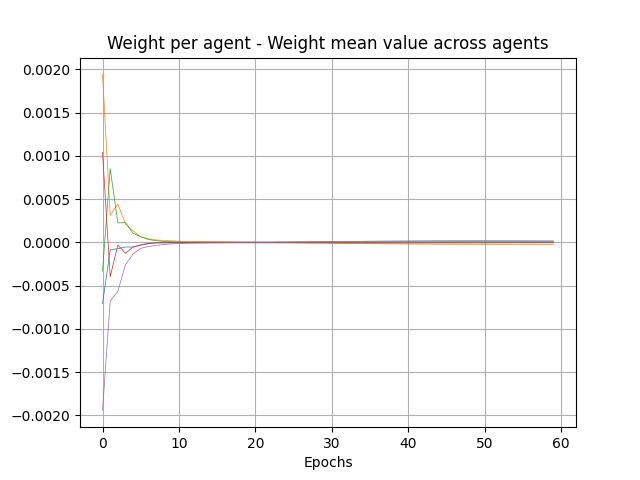
\includegraphics[width=\textwidth]{figs/test1/Single_weight-60}
	\caption{Weight evolution (first 60 epochs)}
	\end{subfigure}
\caption{Evolution of a single weight.}
\label{test1_var}
\end{figure}

\section{Second test}
In the second experiment we check whether the target digit impacts the network behaviour, in particular we use the digit 7 as a target instead of the digit 8 used in the first experiment. From the following plots \ref{test2_loss} and \ref{test2_var} we notice that the decrease both in the cost and gradients magnitude is very similar across these experiments, which indicates a good generalization ability of the network, i.e., that the network is capable of distinguishing different input digits.

\begin{figure}[h]
\centering
	\begin{subfigure}{0.49\textwidth}	
	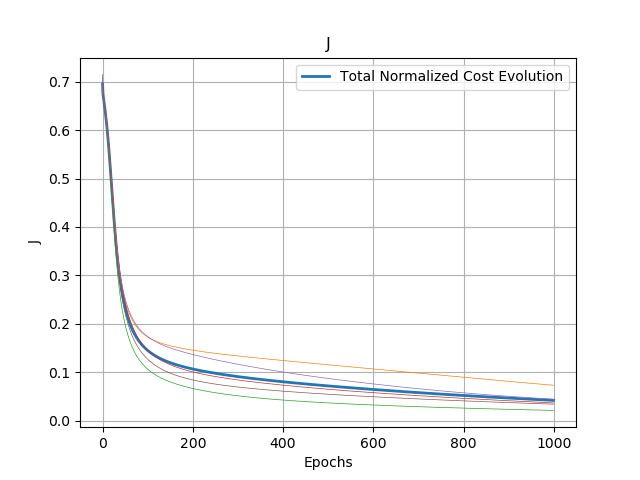
\includegraphics[width=\textwidth]{figs/test2/J.png}
	\caption{Cost evolution}
	\end{subfigure}
\hfill
	\begin{subfigure}{0.49\textwidth}	
	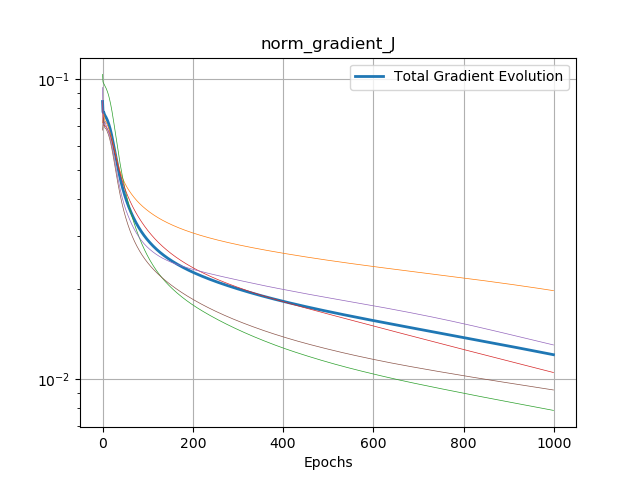
\includegraphics[width=\textwidth]{figs/test2/norm_gradient_J.png}
	\caption{Gradients evolution}
	\end{subfigure}
 \caption{Evolution of the cost function and norm of the gradients.}
\label{test2_loss}
\end{figure}

We may also note a slightly slower convergence to consensus in this second experiment, in fact the amplitude of the first oscillations \ref{test2_var}(b) is slightly bigger than in the first experiment. 

\begin{figure}[h]
\centering
	\begin{subfigure}{0.49\textwidth}	
	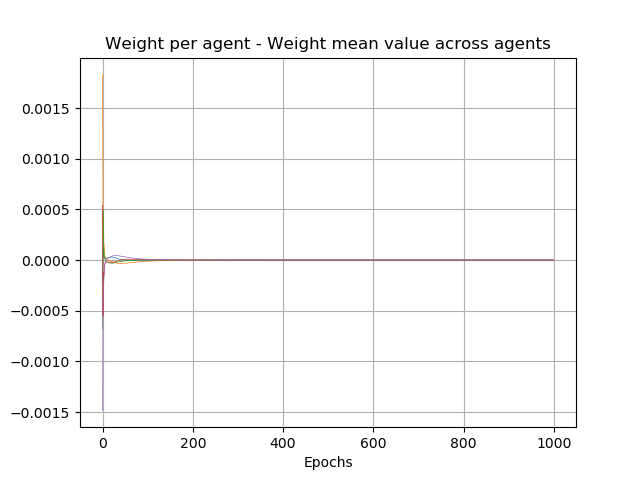
\includegraphics[width=\textwidth]{figs/test2/Single_weight.png}
	\caption{Weight evolution}
	\end{subfigure}
\hfill
	\begin{subfigure}{0.49\textwidth}	
	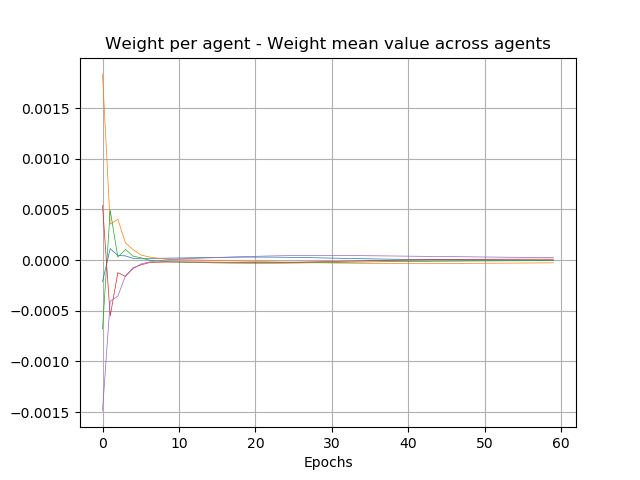
\includegraphics[width=\textwidth]{figs/test2/Single_weight-60.png}
	\caption{Weight evolution (first 60 epochs)}
	\end{subfigure}
\caption{Evolution of a single weight.}
\label{test2_var}
\end{figure}

We have repeated the test previously explained giving as target the different available digits: in the following we show the results obtained in terms of accuracy.
The simulations have been obtained with $5$ agents connected with a cycle graph, and a step-size of $1e^{-2}$.

\begin{center}
\begin{tabular}{|c|c|}
\hline
Target digit & Accuracy \\
\hline
0 & 97.66\% \\
1 & 96.88\% \\
2 & 94.92\% \\
3 & Row 4 \\
4 & Row 5 \\
5 & Row 6 \\
6 & Row 7 \\
7 & Row 8 \\
8 & Row 9 \\
9 & Row 10 \\
\hline
\end{tabular}
\end{center}

\section{Third test}
We have done, as last test, a check on how much the shape of the communication graph influences the velocity (in terms of epochs) required in order to reach the consensus.
We have tested three different graphs:
\begin{itemize}
\item cycle graph
\item star graph
\item path graph
\end{itemize}

As expected the number of epochs required to reach consensus is smaller in case of a better connected graph such as the cycle, while it's bigger for the star graph.
We can also observe that, for example in the star graph, the agent in the "middle" of the connection (agent $2$ with the green line) is the faster to reach consensus since it has a lot of neighbors with respect to the agents on the branches of the graph.

\begin{figure}[h]
\centering
	\begin{subfigure}{0.49\textwidth}	
	\includegraphics[width=\textwidth]{/Test_cycle_200/Weights_difference}
	\caption{Weights evolution}
	\end{subfigure}
\hfill
	\begin{subfigure}{0.49\textwidth}	
	\includegraphics[width=\textwidth]{/Test_cycle_200/Single_weight}
	\caption{Single weight (last neuron) evolution}
	\end{subfigure}
\caption{Evolution of a weights to consensus with \textbf{cycle} graph}
\label{cycle_test}
\end{figure}

\begin{figure}[h]
\centering
	\begin{subfigure}{0.49\textwidth}	
	\includegraphics[width=\textwidth]{/Test_path_200/Weights_difference}
	\caption{Weights evolution}
	\end{subfigure}
\hfill
	\begin{subfigure}{0.49\textwidth}	
	\includegraphics[width=\textwidth]{/Test_path_200/Single_weight}
	\caption{Single weight (last neuron) evolution}
	\end{subfigure}
\caption{Evolution of a weights to consensus with \textbf{path} graph}
\label{path_test}
\end{figure}

\begin{figure}[h]
\centering
	\begin{subfigure}{0.49\textwidth}	
	\includegraphics[width=\textwidth]{/Test_star_200/Weights_difference}
	\caption{Weights evolution}
	\end{subfigure}
\hfill
	\begin{subfigure}{0.49\textwidth}	
	\includegraphics[width=\textwidth]{/Test_star_200/Single_weight}
	\caption{Single weight (last neuron) evolution}
	\end{subfigure}
\caption{Evolution of a weights to consensus with \textbf{star }graph}
\label{path_test}
\end{figure}




\chapter{Formation Control} 
 In the second task we were asked to implement in ROS2 a discrete-time version of a \textbf{formation control law} for a team of $N$ robots.

\section{Distance-based formation}
The aim of the task was to obtain a desired geometric formation among a group of $N$ autonomous agents, by acting on the relative positions of agents.

\bigskip
The desired formation can be encoded in terms of an undirected graph, called \textit{formation graph}, whose set of vertices is indexed by the team agents $\mathcal{N} =\{ 1, \cdots, N\}$, and whose set of edges $E=\{(i,j) \in \mathcal{N} \times \mathcal{N} | \, j \in \mathcal{N}_i\}$ contains pairs of agents. Each edge $(i,j) \in E$ is assigned a scalar parameter $d_{ij} = d_{ji} > 0$, representing the distance at which agents $i,j$ should converge to. 

An example could be a predefined formation with hexagon shape with the following \textit{distances matrix}:
\begin{equation}
d_{ij} =
\begin{bmatrix}
0 & l & 0 & d & h & l \\
l & 0 & l & 0 & d & 0 \\
0 & l & 0 & l & 0 & d \\
d & 0 & l & 0 & l & 0 \\
h & d & 0 & l & 0 & l \\
l & 0 & d & 0 & l & 0
\end{bmatrix}
\end{equation}
The desired distance value serve as reference value for the control law. The control law computes control signals for each agent based on its current position and the position of the neighboring agents, aiming to drive the agents towards the desired formation.
The neighbors of a certain agent $i$ can be extracted from the $i$-th row of the distances matrix, by taking the indexes of the elements with $d_j > 0$.

By denoting the position of agent $i \in \{1, \cdots, N\}$ at time $t>0$ with $x_i(t) \in \mathbb{R}^3$, one way to approach distance-based formation control involves the usage of \textbf{potential functions}, similar to the following one:
\begin{equation}
V_{ij}(x)  = \frac{1}{4} \bigg( \lVert x_i - x_j \rVert^2 - d_{ij}^2 \bigg)^2
\label{Formation_potential}
\end{equation}

This kind of potential function represents the energy associated with the relative positions of the agents. By minimizing this potential function, the agents can achieve and maintain the desired formation.
As a consequence, the control law we have implemented for each agent $i$ is the following:
\begin{equation}
\dot{x}_i(t) = f_i(x(t)) = - \sum_{j \in \mathcal{N}_i} \bigg( \lVert x_i - x_j \rVert^2 - d_{ij}^2 \bigg) (x_i - x_j )
\label{Dynamics_no_collision_avoidance}
\end{equation}

Since we were required to work in discrete time, we denote with $p_i^k \in \mathbb{R}^3$ the discretized version of $x_i(t)$ at iteration $k \in \mathbb{N}$ and, once we have computed the dynamics update for agent $i$ we discretize it with Euler formula in the following way:
\begin{equation}
p_i^{k+1} = p_i^{k} + \Delta f_i(p^k)
\end{equation}
where $\Delta > 0$ is the sampling period.

\section{ROS2 implementation}
The solution proposed in previous section has been implemented in ROS2 environment with a code written in Python language.

\bigskip
By means of a launch file (named \texttt{formation\_control.launch.py}) we can generate the desired number of agents and give them the required informations in order to accomplish the target formation. In particular for each agent the launch file generates a ROS2 node that executes the file named \texttt{the\_agent.py}. Each node gets the following main parameters from the launch file:
\begin{itemize}
\item id: a number from $0$ to $N$ associated to the agent's identity
\item initial position, randomly generated
\item distances: each agent gets only "its" row of the distances matrix. In this way it will be able to know who are its neighbors and the distances he has to keep from them in the desired configuration
\item maximum number of dynamics update
\end{itemize}
This file manages the dynamic evolution of the agent and the communication with the other ones (the neighbors' ones). For what regards the communication, we have used a publisher-subscriber protocol implemented in ROS2: each node communicates its position only to its neighbors. The communication between nodes is made using a topic for each edge defined in the formation graph. In order to write to a topic or to read from it, the node must know the name of the topic he want to access.

\bigskip
We have developed also a plotter agent (\texttt{the\_plotter.py}) that can read from its topic the actual positions of all the other agents in order to visualize the evolution of the trajectories of the whole formation.

For what regards the simulation of the team behaviour we have used RViz.

\subsection{Results}
In the following we can see some results obtained during the simulation of the \texttt{formation\_control} package. 
We have tested several formation-shapes that involve different number of agents.


\begin{figure}[h]
\centering
	\begin{subfigure}{0.49\textwidth}	
	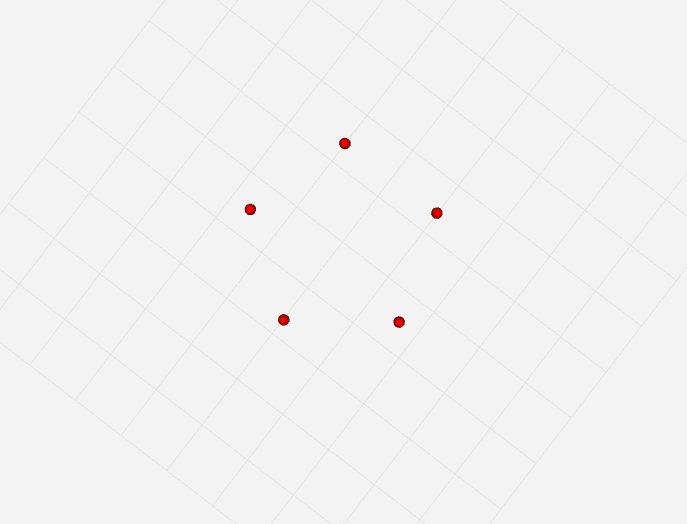
\includegraphics[scale=0.24]{pentagon_rviz}
	\caption{RViz visualization}
	\end{subfigure}
\hfill
	\begin{subfigure}{0.49\textwidth}	
	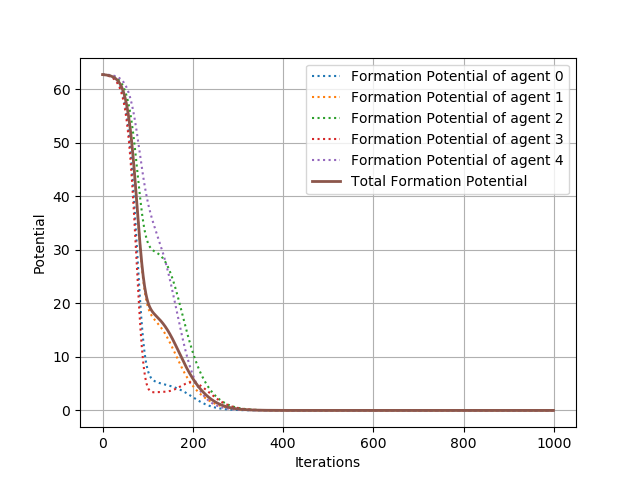
\includegraphics[scale=0.42]{Formation_potential_pentagon}
	\caption{Formation potential plot}
	\end{subfigure}
\caption{Pentagon formation with $5$ agents}
\label{Pentagon}
\end{figure}

\begin{figure}
\centering
	\begin{subfigure}{0.49\textwidth}	
	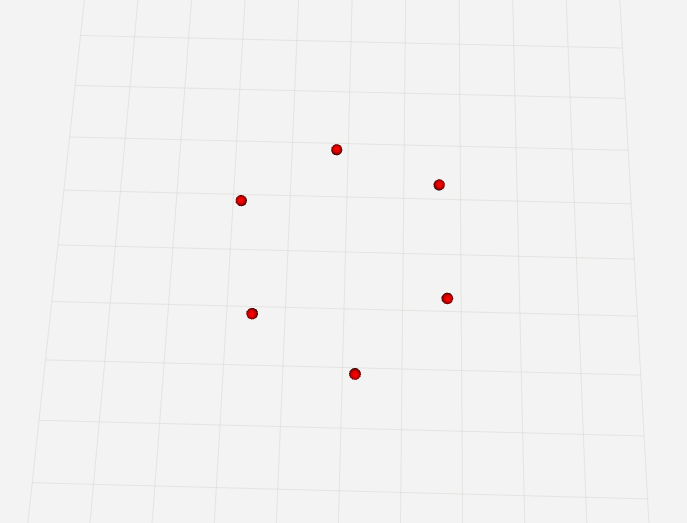
\includegraphics[scale=0.24]{hexagon_rviz}
	\caption{RViz visualization}
	\end{subfigure}
\hfill
	\begin{subfigure}{0.49\textwidth}	
	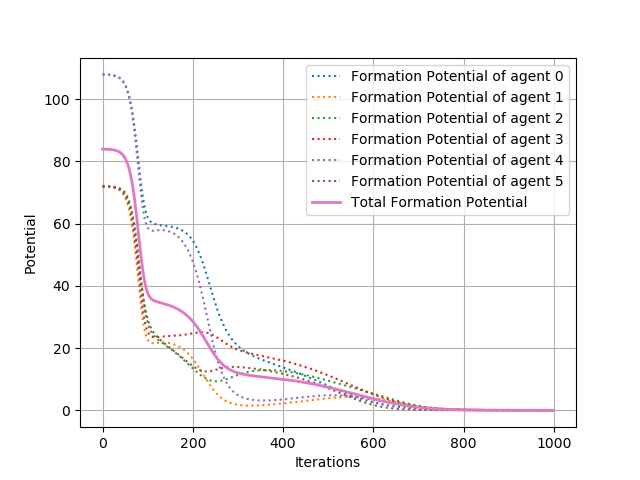
\includegraphics[scale=0.42]{Formation_potential_hexagon}
	\caption{Formation potential plot}
	\end{subfigure}
\caption{Hexagon formation with $6$ agents}
\label{Hexagon}
\end{figure}

\begin{figure}
\centering
	\begin{subfigure}{0.48\textwidth}	
	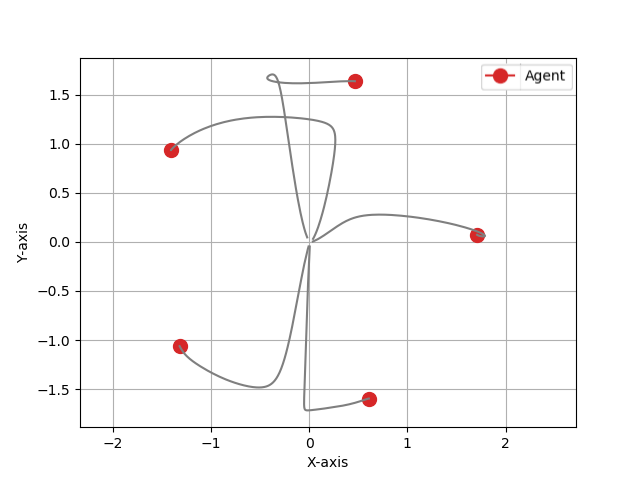
\includegraphics[scale=0.43]{Pentagon_path}
	\caption{Paths for pentagon formation}
	\end{subfigure}
\hfill
	\begin{subfigure}{0.48\textwidth}	
	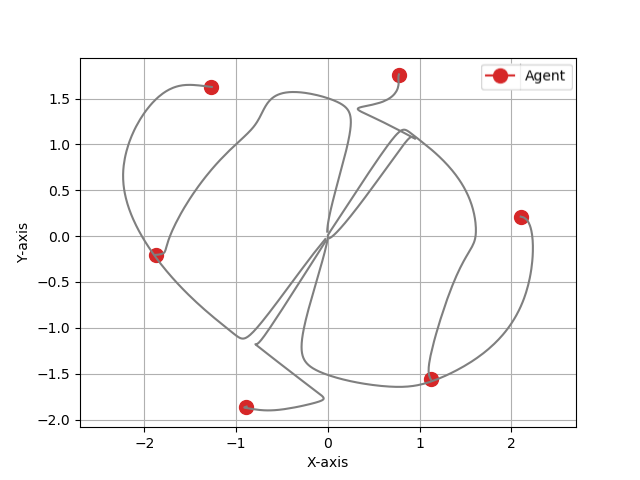
\includegraphics[scale=0.43]{Hexagon_path}
	\caption{Paths for hexagon formation}
	\end{subfigure}
\caption{Paths followed by agents to reach formation}
\label{Paths}
\end{figure}

First of all we have tried 2D-formations like a pentagon and an hexagon, the results are represented respectively in figure \ref{Pentagon} and \ref{Hexagon}. We have initialized the agent's positions randomly and close to zero for the $x$ and the $y$ dimensions, while $z$ position has been initialized equal to zero. Since our target formation is planar, the $z$ remains always equal to zero during the whole evolution.
We show both the final RViz visualization and the potential evolution during the iterations: for the single agents and for the whole formation. The potential diminishes along the iterations while the agents reach the desired configuration. 
For these formations we have also represented in figure \ref{Paths} the paths the single agents follow during the time evolution in order to accomplish the formation.

\begin{figure}
\centering
	\begin{subfigure}{0.49\textwidth}	
	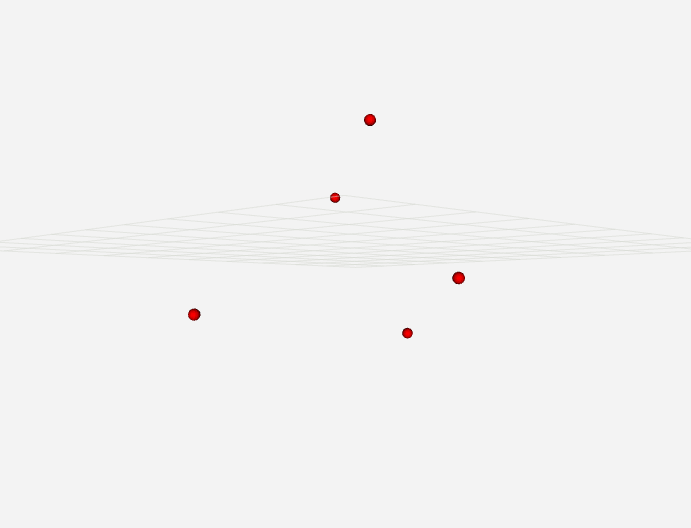
\includegraphics[scale=0.24]{piramid_rviz}
	\caption{RViz visualization}
	\end{subfigure}
\hfill
	\begin{subfigure}{0.49\textwidth}	
	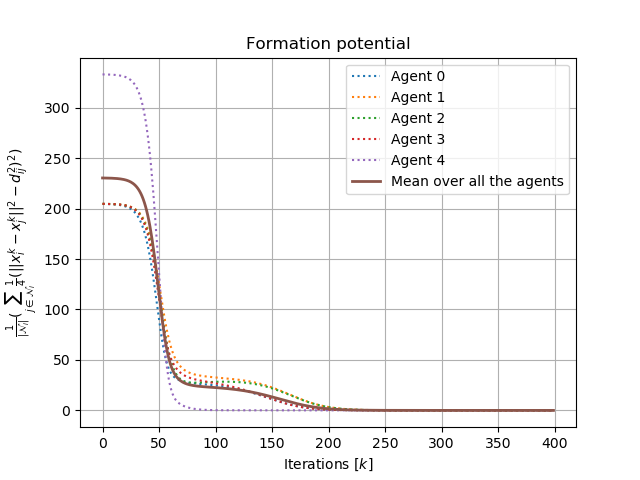
\includegraphics[scale=0.42]{Formation_potential_piramid}
	\caption{Formation potential plot}
	\end{subfigure}
\caption{Square-based piramid with $5$ agents}
\label{Piramid}
\end{figure}

After that, we have tried a 3D-formation, a square-based piramid. In order to do that we have initialized all the $x$, $y$ and $z$ positions close to zero. In figure \ref{Piramid} we can see the results obtained with simulations. The plane the "base-agents" chose, changes from one simulation to the others since we don't have any constraint in this sense.


\section{Collision avoidance}
In formation control, the control laws typically consists of two components: attraction and repulsion. The attraction component pulls the agents towards their desired positions relative to their neighbors, while the repulsion component prevents collision by creating a repulsive force when the agents get too close to each other.

\begin{figure}[h]
\centering
	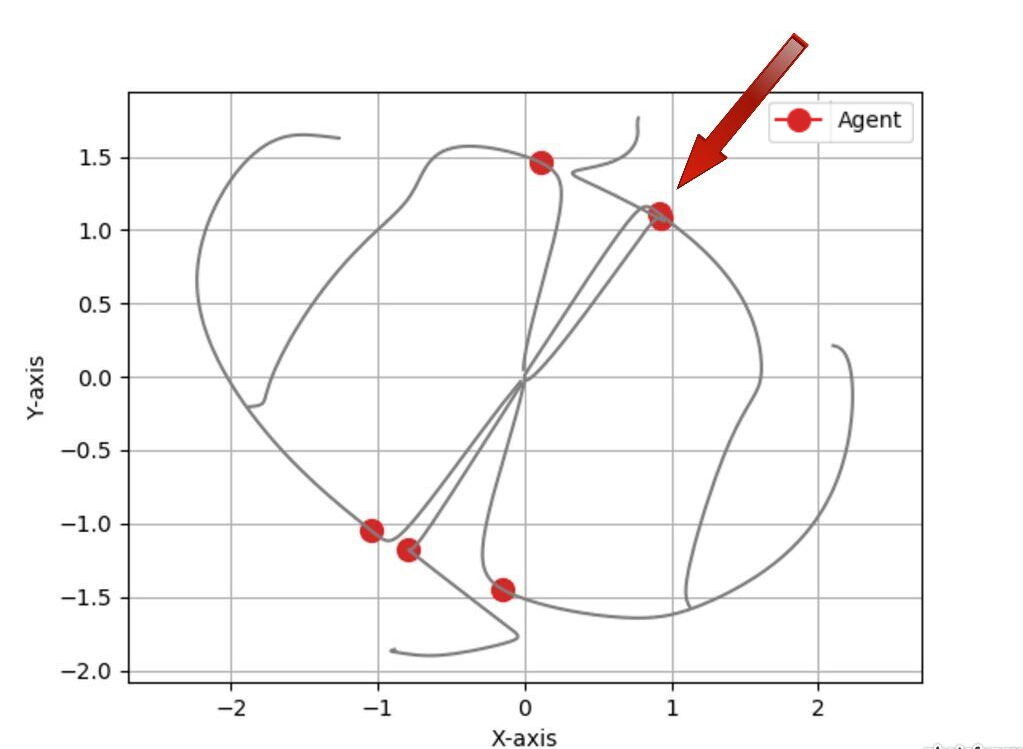
\includegraphics[scale=0.25]{Collision}
	\caption{Collision among two agents during hexagon formation}
	\label{Collision}
\end{figure}

The control law that models the agent's dynamics up to now, had just one component, the one linked to the \textit{formation potential}, formula \ref{Formation_potential}, this was not enough in order to avoid collision among agents (as we can see in figure \ref{Collision}). 

\bigskip
For this reason the \textbf{task 2.2} asked to introduce a second potential to avoid agent's collision. In order to do that the following proper barrier function has been used:
\begin{equation}
V_{ij}(x) = - \log( \lVert x_i - x_j \rVert ^2)
\label{Collision_barrier}
\end{equation}


As a result, the control law has a new term due to this potential that is the following one:
\begin{equation}
\dot{x}_i(t) = - 2\sum_{j \in \mathcal{N}_i} \frac{(x_i-x_j)}{\bigg( \lVert x_i - x_j \rVert^2 - d_{ij}^2 \bigg)}
\end{equation}

And the total control law becomes:
\begin{equation}
\dot{x}_i(t) = - \sum_{j \in \mathcal{N}_i} \bigg( \lVert x_i - x_j \rVert^2 - d_{ij}^2 \bigg) (x_i - x_j ) - 2 \frac{(x_i-x_j)}{\bigg( \lVert x_i - x_j \rVert^2 - d_{ij}^2 \bigg)}
\label{Dynamics_with_collision_avoidance}
\end{equation}

\subsection{Results}
\begin{figure}[h]
\centering
	\begin{subfigure}{0.49\textwidth}	
	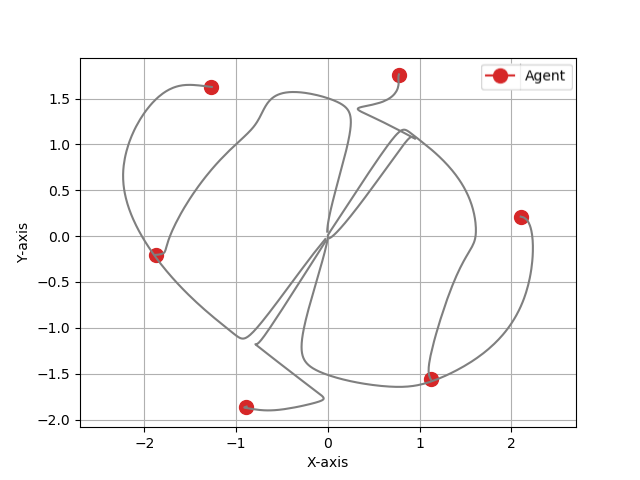
\includegraphics[scale=0.42]{Hexagon_path}
	\caption{Path followed by agents without collision avoidance term}
	\end{subfigure}
\hfill
	\begin{subfigure}{0.49\textwidth}	
	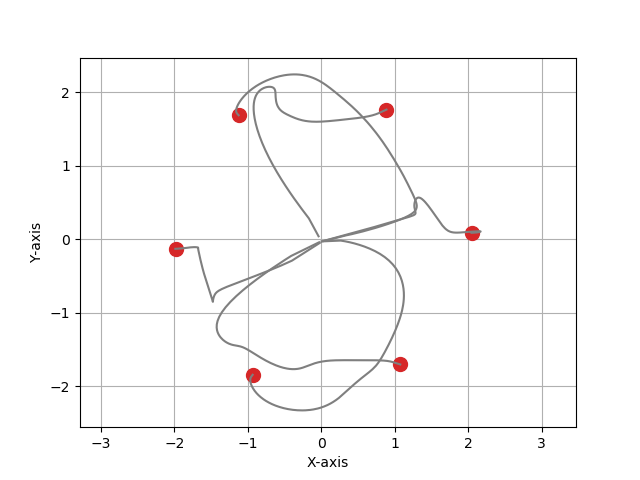
\includegraphics[scale=0.42]{Hexagon_path_collision}
	\caption{Path followed by agents with collision avoidance term}
	\end{subfigure}
\caption{Comparison among paths with and without collision avoidance term}
\label{Paths_comparison}
\end{figure}

In figure \ref{Paths_comparison} we can see the different shape of the paths followed by the agents in order to reach the same hexagon formation. The plot on the left shows the paths due to the dynamic evolution expressed in formula \ref{Dynamics_no_collision_avoidance} (the one without the collision avoidance term), while the plot on the right shows the behaviour due to the introduction of collision avoidance term (formula \ref{Dynamics_with_collision_avoidance}).

\begin{figure}[h]
\centering
	\begin{subfigure}{0.49\textwidth}	
	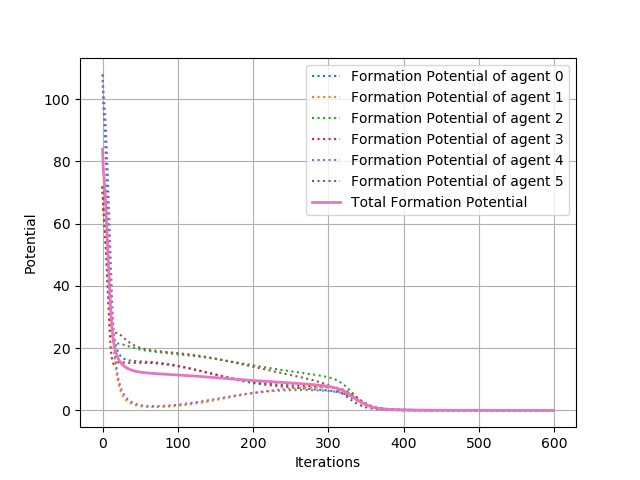
\includegraphics[scale=0.42]{Formation_potential_hexagon_collision}
	\caption{Formation potential (attraction) term}
	\end{subfigure}
\hfill
	\begin{subfigure}{0.49\textwidth}	
	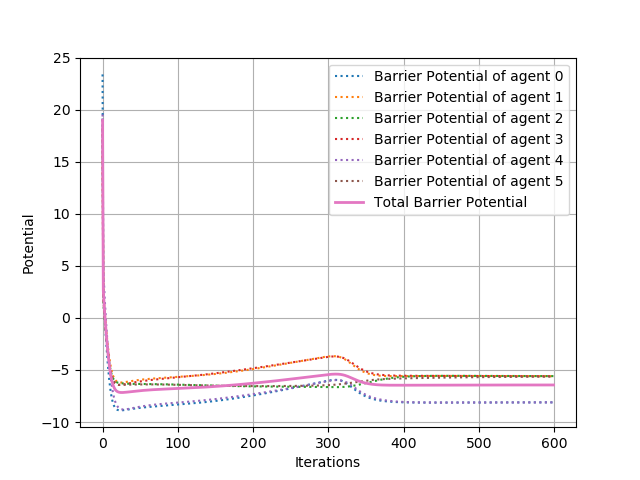
\includegraphics[scale=0.42]{Barrier_potential_hexagon_collision}
	\caption{Barrier potential (repulsion), collision avoidance term}
	\end{subfigure}
\caption{Potential contribution in hexagon formation with collision avoidance}
\label{Potentials_with_collision}
\end{figure}

In figure \ref{Potentials_with_collision} we can see the evolution of the two contributions of the overall potential function. The formation potential, the attractive one that pulls the agents toward the desired formation, diminishes but we can see a "flat area" when the agents goes too close to some neighbors. Accordingly, the barrier potential that repels the agents from neighbors, has a peak.

\section{Moving formation and leaders control}
At this point robots are partitioned in two groups, namely leaders and followers. The objective of \textbf{task 2.3} is to control the translation and/or the rotation of the formation (by giving proper inputs to the leaders) while maintaining the chosen pattern.
Distance constrains  are invariant to both translation and rotation of the formation, so the distance-based approach can be applied to realize translational and rotational formation maneuvers. 

We have modified the \texttt{formation\_control.launch.py} in order to pass to the \texttt{the\_agent.py} file the information about their identity (leader or follower) and about the motion the leaders have to accomplish.

\begin{figure}[h]
\centering
	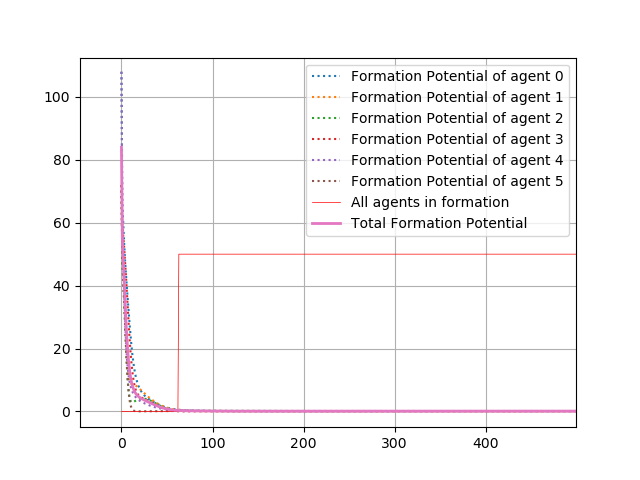
\includegraphics[scale=0.4]{Formation_check}
	\caption{Check on the formation accomplishment}
	\label{Check}
\end{figure}

\bigskip
We use the \texttt{the\_plotter} agent as a "supervisor" that tells all the agents when the target formation has been reached. Once all the agents are in formation the leaders start moving. As a trigger condition the supervisor checks when the potentials' derivatives of all the agents are smaller then a certain threshold. At this moment, he notifies all the agents the formation has been reached and so, the leaders can start moving. This threshold value depends on the formation shape we chose. In figure \ref{Check} the red line represents this notification criterion.

\bigskip
From this moment on, the dynamics evolution changes: the followers continue with the same motion, trying to maintain the formation, while the leader's dynamic has two contributions, the formation one and the motion we have decided them to follow. Both have also the collision avoidance term.

\begin{figure}[h]
\centering
	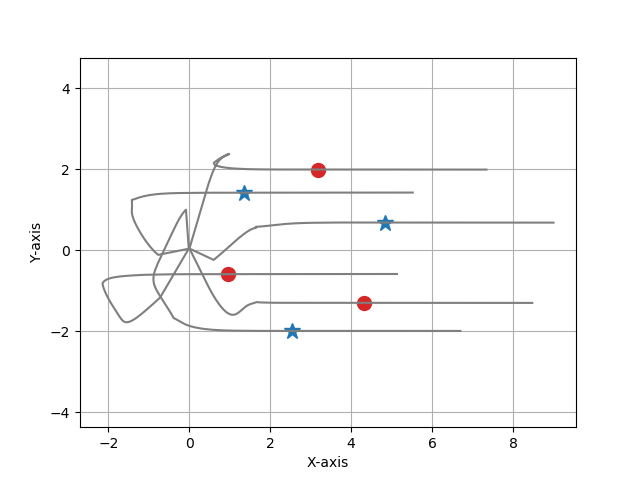
\includegraphics[scale=0.5]{Moving_hexagon_formation_linear}
	\caption{Motion of the formation along the $x$-axis}
	\label{Formation_motion_lin}
\end{figure}

Figure \ref{Formation_motion_lin} represents the motion of the formation along the $x$-axis due to a constant input assigned to leaders' dynamic. The leaders are represented as the blue stars.

\begin{figure}[h]
\centering
	\begin{subfigure}{0.49\textwidth}	
	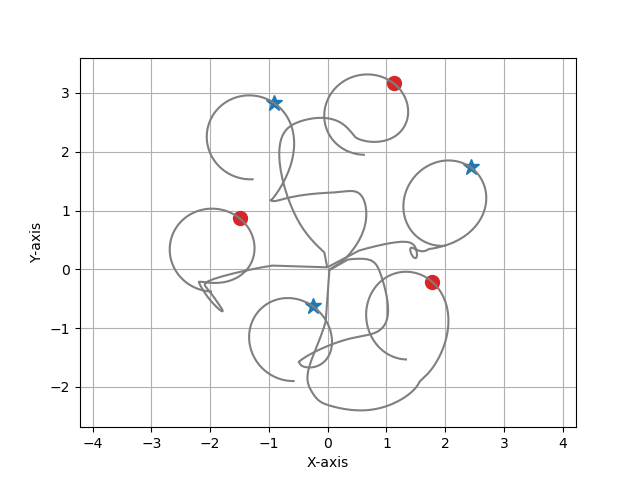
\includegraphics[scale=0.42]{Moving_hexagon_formation_circle_r_2}
	\caption{Moving along a circle of radius $2$}
	\end{subfigure}
\hfill
	\begin{subfigure}{0.49\textwidth}	
	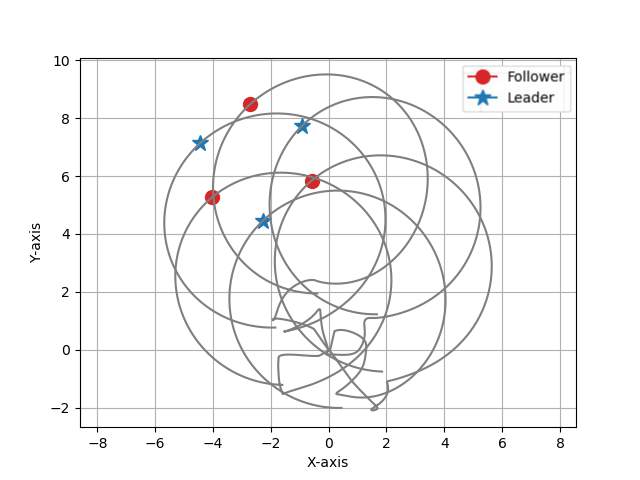
\includegraphics[scale=0.42]{Moving_hexagon_formation_circle_r_5}
	\caption{Moving along a circle of radius $5$}
	\end{subfigure}
\caption{Motion of the formation along a circular path}
\label{Formation_motion_circle}
\end{figure}

\bigskip
We have also tried to give the leaders a proper input in order to accomplish a circular motion during the number of iterations given. In figure \ref{Formation_motion_circle} we can see the motion of the hexagon formation: in the left plot we have given as input a radius equal to $2$ while in the right one the radius is equal to $5$.



\section{Obstacle avoidance}
\textbf{Task 2.4} asked to us to introduce obstacle avoidance in our \texttt{formation\_control} package. Obstacle avoidance in formation control refers to the ability of a group of $N$ coordinated agents to navigate through en environment while maintaining a desired formation and avoiding collision with fixed or moving obstacles. 

In order to accomplish this task we have created a certain number of fixed obstacles as ROS2 nodes. The obstacles gets their position from the launch file and communicate it to the follower agents. 
In \texttt{the\_agent.py} we have still two dynamics: the leaders move according to the assigned input while the followers move according to the formation and trying to avoid obstacles. For this reason we have introduced in the dynamics a potential in order to avoid obstacles:
\begin{equation}
V_{ij}(x) = - \log( \lVert x_i - x_h\rVert ^2)
\label{Obstacles_barrier}
\end{equation}
where $x_h$ denotes the position of the obstacles.

In the following simulation we have given to the leaders of the formation a target position "over" the obstacles: to reach it the formation has to pass inside the window left by the obstacles. 




%%%%%%%%%% Conclusions %%%%%%%%%%
\chapter*{Conclusions}
\addcontentsline{toc}{chapter}{Conclusions} 
In the \textbf{First task} we explored a distributed optimization framework where each individual agent possesses limited knowledge of the global optimization problem. To tackle the classification problem, agents rely solely on local computations and communication with their neighboring agents, without the involvement of a central unit. In order to solve this problem we have implemented a Gradient Tracking algorithm. 
We have obtained good results both in terms of consensus and accuracy of the classification. 

\bigskip
In the \textbf{Second task} we have seen the power of a ROS2 implementation of formation control for a network of N robotic agent, by applying a distance-based control law, and by allowing only local communication with neighbors. We have also seen how the agents are able to follow a predefined trajectory maintaining the formation very well.
We have also explored the possibility of introduce obstacle and collision avoidance between agents and it seems to work very well.

%%%%%%%%%% Bibliography %%%%%%%%%%%

%\bibliographystyle{sample}
%\bibliography{references}{}
%\addcontentsline{toc}{chapter}{Bibliography}


%%%%%%%%%%%%%%%%%%%%%%%%%%%%%%%%%%%%%%

\end{document}